


\tikzset{every picture/.style={line width=0.75pt}} %set default line width to 0.75pt

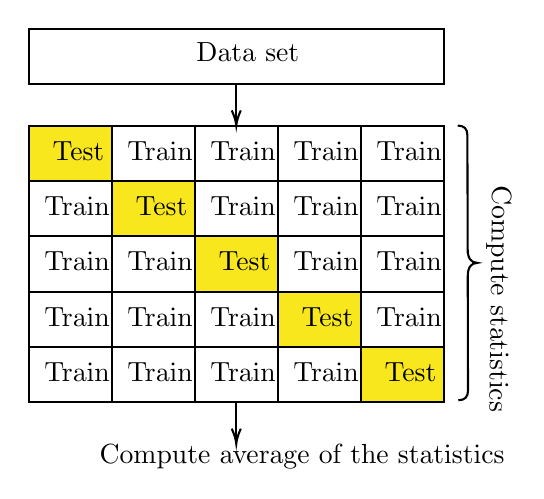
\begin{tikzpicture}[x=0.5pt,y=0.5pt,yscale=-1,xscale=1]
%uncomment if require: \path (0,487); %set diagram left start at 0, and has height of 487

%Shape: Rectangle [id:dp9628831478307318]
\draw   (90,20) -- (390,20) -- (390,60) -- (90,60) -- cycle ;
%Shape: Rectangle [id:dp40247556319098454]
\draw   (150,90) -- (210,90) -- (210,130) -- (150,130) -- cycle ;
%Straight Lines [id:da38673279994063514]
\draw    (240,60) -- (240,88) ;
\draw [shift={(240,90)}, rotate = 270] [color={rgb, 255:red, 0; green, 0; blue, 0 }  ][line width=0.75]    (10.93,-3.29) .. controls (6.95,-1.4) and (3.31,-0.3) .. (0,0) .. controls (3.31,0.3) and (6.95,1.4) .. (10.93,3.29)   ;
%Shape: Brace [id:dp44265578721237586]
\draw   (400.5,288.5) .. controls (405.17,288.49) and (407.49,286.15) .. (407.48,281.48) -- (407.28,199.23) .. controls (407.27,192.56) and (409.59,189.23) .. (414.26,189.22) .. controls (409.59,189.23) and (407.25,185.9) .. (407.23,179.23)(407.24,182.23) -- (407.03,96.98) .. controls (407.02,92.31) and (404.68,89.99) .. (400.01,90) ;
%Shape: Rectangle [id:dp6086176363319614]
\draw  [fill={rgb, 255:red, 248; green, 231; blue, 28 }  ,fill opacity=1 ] (90,90) -- (150,90) -- (150,130) -- (90,130) -- cycle ;
%Shape: Rectangle [id:dp6253670891530648]
\draw   (210,90) -- (270,90) -- (270,130) -- (210,130) -- cycle ;
%Shape: Rectangle [id:dp012463141021535118]
\draw   (270,90) -- (330,90) -- (330,130) -- (270,130) -- cycle ;
%Shape: Rectangle [id:dp03635717517805359]
\draw   (330,90) -- (390,90) -- (390,130) -- (330,130) -- cycle ;
%Shape: Rectangle [id:dp6139521323150046]
\draw   (90,130) -- (150,130) -- (150,170) -- (90,170) -- cycle ;
%Shape: Rectangle [id:dp2734748607023023]
\draw   (210,130) -- (270,130) -- (270,170) -- (210,170) -- cycle ;
%Shape: Rectangle [id:dp7416160208443594]
\draw   (270,130) -- (330,130) -- (330,170) -- (270,170) -- cycle ;
%Shape: Rectangle [id:dp04965387626199025]
\draw   (330,130) -- (390,130) -- (390,170) -- (330,170) -- cycle ;
%Shape: Rectangle [id:dp36390369464546923]
\draw   (90,170) -- (150,170) -- (150,210) -- (90,210) -- cycle ;
%Shape: Rectangle [id:dp0583337342908441]
\draw   (150,170) -- (210,170) -- (210,210) -- (150,210) -- cycle ;
%Shape: Rectangle [id:dp7518796244751725]
\draw   (270,170) -- (330,170) -- (330,210) -- (270,210) -- cycle ;
%Shape: Rectangle [id:dp8731512433065419]
\draw   (330,170) -- (390,170) -- (390,210) -- (330,210) -- cycle ;
%Shape: Rectangle [id:dp3374950674483356]
\draw   (90,210) -- (150,210) -- (150,250) -- (90,250) -- cycle ;
%Shape: Rectangle [id:dp2425800253901771]
\draw   (150,210) -- (210,210) -- (210,250) -- (150,250) -- cycle ;
%Shape: Rectangle [id:dp9764918971023423]
\draw   (210,210) -- (270,210) -- (270,250) -- (210,250) -- cycle ;
%Shape: Rectangle [id:dp3030426321919574]
\draw   (330,210) -- (390,210) -- (390,250) -- (330,250) -- cycle ;
%Shape: Rectangle [id:dp08910405765909535]
\draw   (90,250) -- (150,250) -- (150,290) -- (90,290) -- cycle ;
%Shape: Rectangle [id:dp3282550386553066]
\draw   (150,250) -- (210,250) -- (210,290) -- (150,290) -- cycle ;
%Shape: Rectangle [id:dp25498660930064765]
\draw   (210,250) -- (270,250) -- (270,290) -- (210,290) -- cycle ;
%Shape: Rectangle [id:dp08541585559965792]
\draw   (270,250) -- (330,250) -- (330,290) -- (270,290) -- cycle ;
%Shape: Rectangle [id:dp19772098788401882]
\draw  [fill={rgb, 255:red, 248; green, 231; blue, 28 }  ,fill opacity=1 ] (150,130) -- (210,130) -- (210,170) -- (150,170) -- cycle ;
%Shape: Rectangle [id:dp01839862708870832]
\draw  [fill={rgb, 255:red, 248; green, 231; blue, 28 }  ,fill opacity=1 ] (210,170) -- (270,170) -- (270,210) -- (210,210) -- cycle ;
%Shape: Rectangle [id:dp11813630833655397]
\draw  [fill={rgb, 255:red, 248; green, 231; blue, 28 }  ,fill opacity=1 ] (270,210) -- (330,210) -- (330,250) -- (270,250) -- cycle ;
%Shape: Rectangle [id:dp9995560009248317]
\draw  [fill={rgb, 255:red, 248; green, 231; blue, 28 }  ,fill opacity=1 ] (330,250) -- (390,250) -- (390,290) -- (330,290) -- cycle ;
%Straight Lines [id:da24602633489740156]
\draw    (240,290) -- (240,318) ;
\draw [shift={(240,320)}, rotate = 270] [color={rgb, 255:red, 0; green, 0; blue, 0 }  ][line width=0.75]    (10.93,-3.29) .. controls (6.95,-1.4) and (3.31,-0.3) .. (0,0) .. controls (3.31,0.3) and (6.95,1.4) .. (10.93,3.29)   ;

% Text Node
\draw (105,99) node [anchor=north west][inner sep=0.75pt]   [align=left] {Test};
% Text Node
\draw (159,99) node [anchor=north west][inner sep=0.75pt]   [align=left] {Train};
% Text Node
\draw (209,28) node [anchor=north west][inner sep=0.75pt]   [align=left] {Data set};
% Text Node
\draw (441.01,131.27) node [anchor=north west][inner sep=0.75pt]  [rotate=-90.74] [align=left] {Compute statistics};
% Text Node
\draw (139,318) node [anchor=north west][inner sep=0.75pt]   [align=left] {Compute average of the statistics};
% Text Node
\draw (219,99) node [anchor=north west][inner sep=0.75pt]   [align=left] {Train};
% Text Node
\draw (279,99) node [anchor=north west][inner sep=0.75pt]   [align=left] {Train};
% Text Node
\draw (339,99) node [anchor=north west][inner sep=0.75pt]   [align=left] {Train};
% Text Node
\draw (99,139) node [anchor=north west][inner sep=0.75pt]   [align=left] {Train};
% Text Node
\draw (219,139) node [anchor=north west][inner sep=0.75pt]   [align=left] {Train};
% Text Node
\draw (279,139) node [anchor=north west][inner sep=0.75pt]   [align=left] {Train};
% Text Node
\draw (339,139) node [anchor=north west][inner sep=0.75pt]   [align=left] {Train};
% Text Node
\draw (99,179) node [anchor=north west][inner sep=0.75pt]   [align=left] {Train};
% Text Node
\draw (159,179) node [anchor=north west][inner sep=0.75pt]   [align=left] {Train};
% Text Node
\draw (279,179) node [anchor=north west][inner sep=0.75pt]   [align=left] {Train};
% Text Node
\draw (339,179) node [anchor=north west][inner sep=0.75pt]   [align=left] {Train};
% Text Node
\draw (99,219) node [anchor=north west][inner sep=0.75pt]   [align=left] {Train};
% Text Node
\draw (159,219) node [anchor=north west][inner sep=0.75pt]   [align=left] {Train};
% Text Node
\draw (219,219) node [anchor=north west][inner sep=0.75pt]   [align=left] {Train};
% Text Node
\draw (339,219) node [anchor=north west][inner sep=0.75pt]   [align=left] {Train};
% Text Node
\draw (99,259) node [anchor=north west][inner sep=0.75pt]   [align=left] {Train};
% Text Node
\draw (159,259) node [anchor=north west][inner sep=0.75pt]   [align=left] {Train};
% Text Node
\draw (219,259) node [anchor=north west][inner sep=0.75pt]   [align=left] {Train};
% Text Node
\draw (279,259) node [anchor=north west][inner sep=0.75pt]   [align=left] {Train};
% Text Node
\draw (165,139) node [anchor=north west][inner sep=0.75pt]   [align=left] {Test};
% Text Node
\draw (225,179) node [anchor=north west][inner sep=0.75pt]   [align=left] {Test};
% Text Node
\draw (285,219) node [anchor=north west][inner sep=0.75pt]   [align=left] {Test};
% Text Node
\draw (345,259) node [anchor=north west][inner sep=0.75pt]   [align=left] {Test};


\end{tikzpicture}
